% Going off the Thesis guidelines available here: http://www.lboro.ac.uk/students/welcome/research/codes-of-practice/appendices/
% A4 paper size selected, default is 11pt font, to change to 12pt use [a4paper, 12pt] as option to documentclass
\documentclass[a4paper]{report}

% Some useful packages for including images, colored font, etc.
\usepackage[dvips]{graphicx}
\graphicspath{{Figures/}}

\makeatletter
\def\maxwidth{\ifdim\Gin@nat@width>\linewidth\linewidth\else\Gin@nat@width\fi}
\def\maxheight{\ifdim\Gin@nat@height>\textheight\textheight\else\Gin@nat@height\fi}
\makeatother
\setkeys{Gin}{width=\maxwidth,height=\maxheight,keepaspectratio}
\usepackage{amssymb,amsmath}
\usepackage{longtable}
\usepackage{booktabs}

\usepackage{listings}
\usepackage{xcolor}
 
\definecolor{codegreen}{rgb}{0,0.6,0}
\definecolor{codegray}{rgb}{0.5,0.5,0.5}
\definecolor{codepurple}{rgb}{0.58,0,0.82}
\definecolor{backcolour}{rgb}{0.95,0.95,0.92}
 
\lstdefinestyle{mystyle}{
    backgroundcolor=\color{backcolour},   
    commentstyle=\color{codegreen},
    keywordstyle=\color{magenta},
    numberstyle=\tiny\color{codegray},
    stringstyle=\color{codepurple},
    basicstyle=\ttfamily\footnotesize,
    breakatwhitespace=false,         
    breaklines=true,                 
    captionpos=b,                    
    keepspaces=true,                 
    numbers=left,                    
    numbersep=5pt,                  
    showspaces=false,                
    showstringspaces=false,
    showtabs=false,                  
    tabsize=2
}
 
\lstset{style=mystyle}

\usepackage[numbers]{natbib}

\usepackage{color}
\usepackage{url}
\usepackage{subcaption}

% Global bibliography style
\bibliographystyle{unsrt}

% Set margins in all document to 3.5cm as per guidelines for binding
\usepackage[includeheadfoot,margin=3.5cm]{geometry}

% Used to including pdf files within pages
% use [draft] as option to output empty spaces rather than rendering all pages (useful when including lots of pdfs)
\usepackage{pdfpages}

% Used to produce headers and footers
\usepackage{fancyhdr}
\pagestyle{fancyplain}

% Used for removing title in bibliography sections
\usepackage{titlesec}

% Used to generate lists of abbreviations
\usepackage{nomencl}
\makenomenclature 
\renewcommand{\nomname}{List of Abbreviations}

% To have a separate bibliography per Chapter uncomment this line
% See Introduction/Introduction.tex for example how to include the bibliography
%\usepackage{chapterbib}

% Line spacing defined at 1 and a half. I know it says 1.3 but its 1 and a half.
\linespread{1.3}

% Setup headers and footers
\fancyhf{}
\lhead{\leftmark}
% Center on all pages
% \fancyhead[C]{---Draft---}
% Page number placed on right side on odd pages and left side on even pages
\fancyfoot[RO, LE] {\thepage}


\begin{document}

% Give \subsubsection numbers
\setcounter{secnumdepth}{4}

% Title, Author, Abstract, Acknowledgement, Table of Content, List of Figures, List of Tables and List of Abbreviations
% Front matter of the Thesis
% Title page
% Loughborough University Thesis Access Form
% Loughborough University Certificate of Originality
% Abstract
% Acknowledgements
\title{\bf Building BT Network}

\author{by\\
Zhihao DAI\\
Yunsong ZHANG\\
Huijing LEI\\
Changrong CHEN\\
Yan HUANG\\
\\
{\bf 19COP502 Building Secure Networks}\\
{\bf Lab Report}\\
\\
Loughborough University\\
\\
\copyright
\hspace{1 dd} BT NETWORK 2019\\
\\
Nov. 2019
}
\date{} % Used to remove date from title so it can be set at any date rather than the current date

\maketitle

% Set page numbers to roman numerals for front matter
\pagenumbering{roman}

% % PDF exports of Word Documents available (Exported August 2012)
% % Thesis Access Form
% 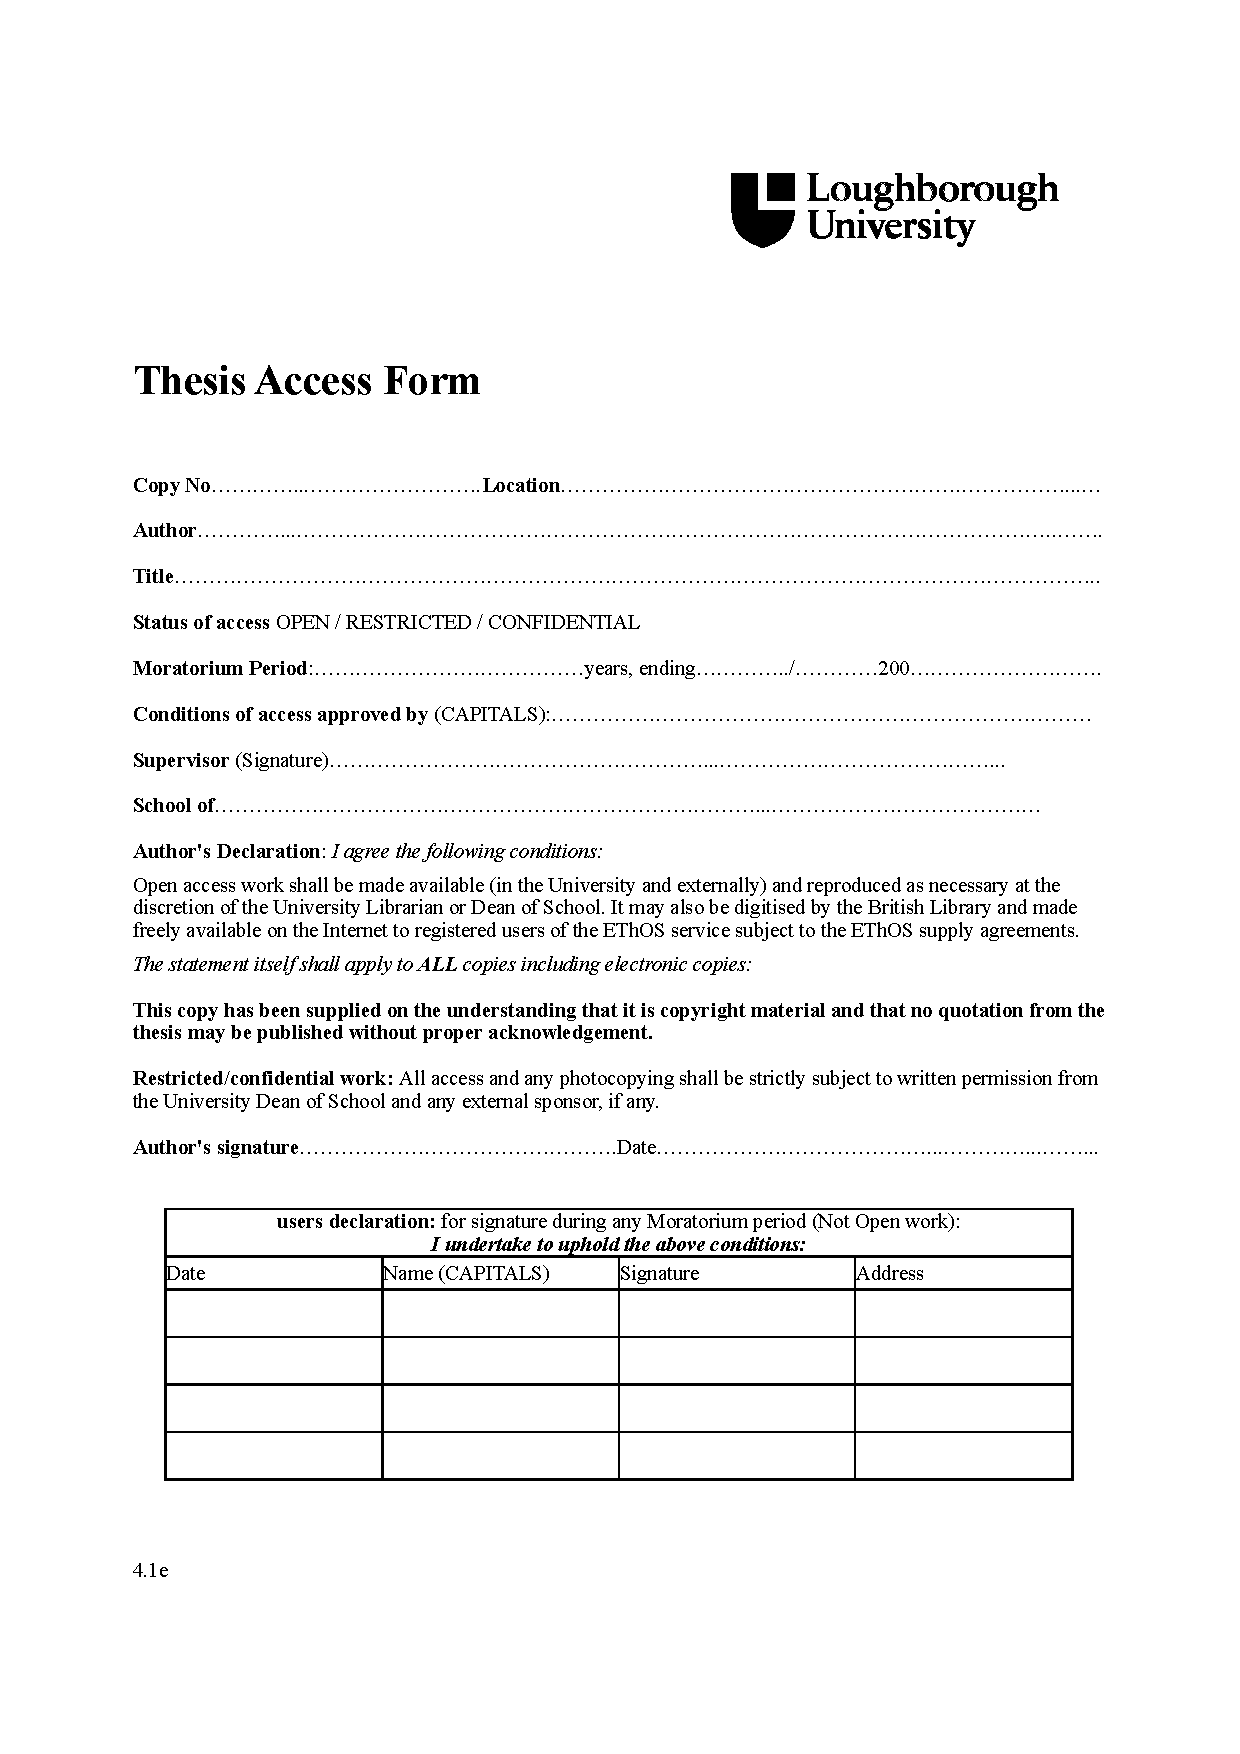
\includepdf[pages=1, pagecommand=, templatesize={5in}{10in}]{Front/LU/access.pdf}
% % Certificate of Originality
% 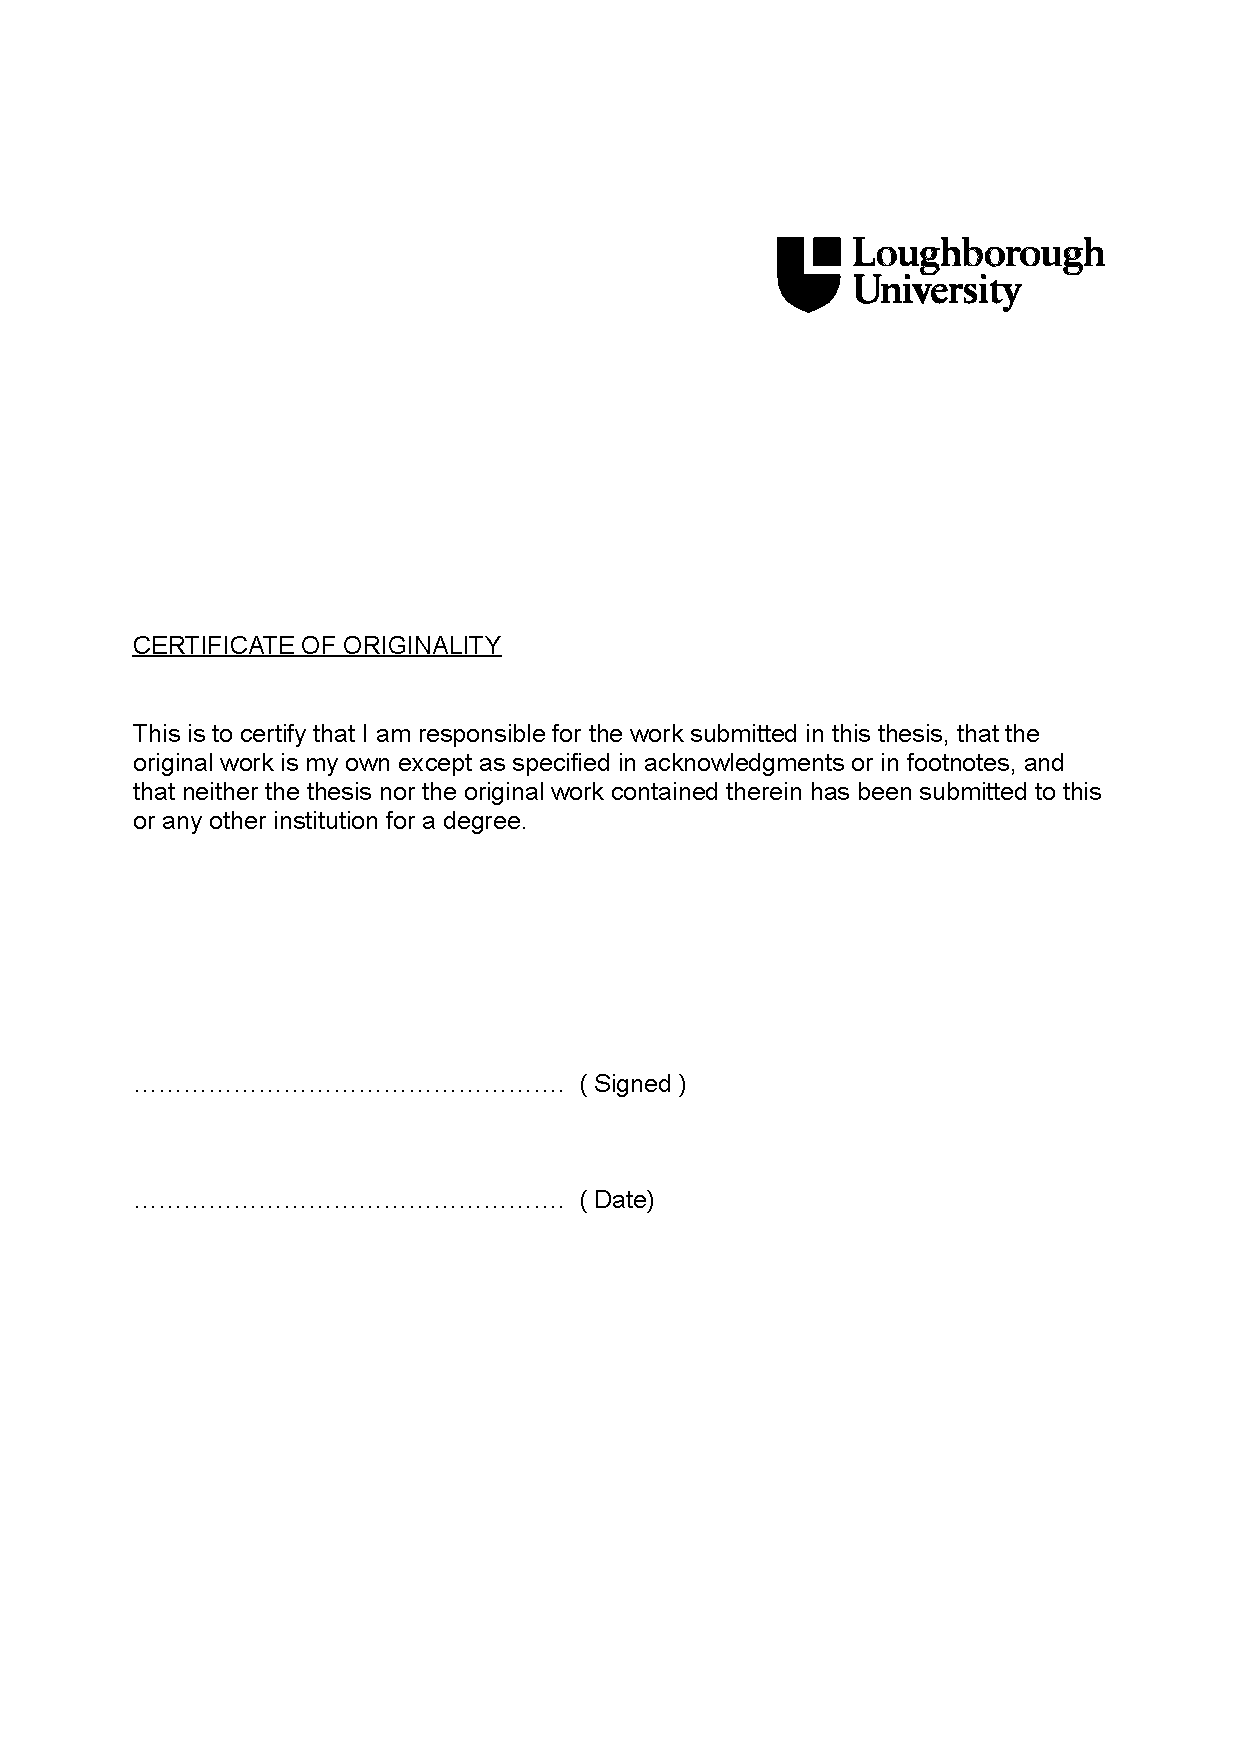
\includepdf[pages=-, pagecommand=, templatesize={5in}{10in}]{Front/LU/origin.pdf}

% Abstract
\addcontentsline{toc}{chapter}{Abstract}
\chapter*{Abstract}
TODO


% % Acknowledgements
% \addcontentsline{toc}{chapter}{Acknowledgements}
% \chapter*{Acknowledgements}
% Acknowledgement section.

% Set the depth for your table of content
% Currently set at 2 (Chapter, Section, Subsection)
\setcounter{tocdepth}{2}
% Include a table of content
\tableofcontents

% Include a list of figures
\addcontentsline{toc}{chapter}{List of Figures}
\listoffigures

% Include a list of tables
\addcontentsline{toc}{chapter}{List of Tables}
\listoftables

% Include a list of abbreviations using nomenclature package
%\addcontentsline{toc}{chapter}{List of Abbreviations}
%\printnomenclature[3cm] 

\newpage

% Set page numbering to arabic for body of Thesis
\pagenumbering{arabic}


% To keep everything neat I included each chapter as a separate .tex file
% Each contains a single chapter, they include all the settings defined in this .tex file
% Allows easier moving around of chapters

% Use \include{<path to .tex file>} to include documents
% For example
\chapter{Introduction}
\label{chap:introduction}

In this lab, our team set out to build BT Network, a small version of Tier-2 Internet Service Provider (ISP) located at Haslegrave Building, from scratch. Despite its limitations in terms of size and Internet access, we can proudly attest that BT Network is one of the leading providers at Haslegrave Building.

BT network is a Autonomous System (AS) as a whole and the AS Number is \texttt{2030}. Its domain name is \texttt{bt.lboro} .


\chapter{Network Architecture}
\label{chap:architecture}

\section{Network Diagram}

\subsection{Description}

\subsection{IP Addresses and Interfaces}

\subsection{Connections to Neighbor ISPs}



\section{IP Addresses of Interfaces}

\subsection{Design}

\subsection{Implementation}

\subsection{Evaluation}

\subsection{Commentary}


\chapter{Routing Protocols in the Network}
\label{chap:routing}




\chapter{Applications in the Network}
\label{chap:applications}

\section{Secure Remote Access to Routers through SSH}

\subsection{Design}

Accessing the routers through the physical "console" port is inconvenient and dangerous. Thus, remote acess through Secure Shell (SSH) protocol to routers is needed. 

In our network, we enable remote SSH access on all 3 routers. We use seperate combinations of username and password on each router to ensure the independence of security of each router.

In addition, we set up SSH public key authentication on Laptop 1 (BT001), which allows the root user on the laptop to login in to all routers without entering passwords.

\subsection{Implementation}

We first set up remote SSH access as instructed in Reference Guide on all 3 routers. Below is the configuration commands for Router 1 (BT-R001).

\begin{lstlisting}
hostname BT-R001
ip domain name bt.lboro
username r001 priv 15 secret <secret>
line vty 0 4
transport input ssh telnet
login local

ip ssh version 2
crypto key generate rsa general-keys
ip ssh dh min size 4096
\end{lstlisting}

We then generate a pair of public and private keys on Laptop 1 (BT001).

\begin{lstlisting}
ssh-keygen
\end{lstlisting}

After that, the pair of keys is written into files
\texttt{\textasciitilde{}/.ssh/id\_rsa} and
\texttt{\textasciitilde{}/.ssh/id\_rsa.pub} . We use the generated
public key ( \texttt{id\_rsa.pub} ) to set up SSH public key
authentication on all 3 routers.

\begin{lstlisting}
ip ssh pubkey-chain
username r001
key-string
\end{lstlisting}

\subsection{Evaluation}

Once remote SSH access is set up on 3 routers, we should be able to access them on Laptop 1 (BT001) without entering the password using the following commands.

\begin{lstlisting}[language=sh]
# access Router 1
ssh r001@23.0.0.1 
# access Router 2
ssh r002@23.0.0.50
# access Router 3
ssh r003@23.0.0.33
\end{lstlisting}

Screenshots of successful remote access to all 3 routers are shown in Figure \ref{fig:ssh}.

\begin{figure*}[t!]
    \centering
    \begin{subfigure}[t]{0.3\textwidth}
        \centering
        \includegraphics[width=\linewidth]{ssh1}
        \caption{Router 1 (BT-R001)}
    \end{subfigure}
    ~ 
    \begin{subfigure}[t]{0.3\textwidth}
        \centering
        \includegraphics[width=\linewidth]{ssh2}
        \caption{Router 2 (BT-R002)}
    \end{subfigure}
    ~ 
    \begin{subfigure}[t]{0.3\textwidth}
        \centering
        \includegraphics[width=\linewidth]{ssh3}
        \caption{Router 3 (BT-R003)}
    \end{subfigure}
    \caption{Sucessful remote SSH access to all 3 routers from Laptop 1 (BT001).}
    \label{fig:ssh}
\end{figure*}


\subsection{Commentary}

\subsubsection{Problem: Maximum Limit of Characters per Line}

When we tried to set up SSH public key authentication on routers, we failed at our initial attempt. It turned out that Cisco router has maximum limit of characters for each command line. Thus, a public key in a single long line was not accepted by the router. 

To solve this problem, we then used \texttt{fold} command to split the public key into multiple lines before re-uploading the key and SSH public key authentication was successfully set up on the router.


\section{World Wide Web Service}

\subsection{Design}

\subsection{Implementation}

\subsection{Evaluation}

\subsection{Commentary}



\section{Domain Name System Service}

\subsection{Design}

\subsection{Implementation}

\subsection{Evaluation}

\subsection{Commentary}


\section{Email Service}

\subsection{Design}

\subsection{Implementation}

\subsection{Evaluation}

\subsection{Commentary}

\chapter{Discussion}
\label{chap:discussion}

\section{Conclusions}
Several conclusions can be drawn from this lab.

\begin{enumerate}
\item
  BT Network, a small Tier-2 ISP, has been built and well tested. 
\item
  BT Network provides both intra-domain and inter-domain Internet connection to its users. It serves common Internet applications including Web, DNS and Email as well.
\item
  BT Network forms and implements business relationships with neighbouring ISPs.
\item
  Both IS-IS and BGP routing protocols can provide alternative route(s) to the destination when one of the physicial links is down.  
\end{enumerate}


\section{Further Work}

For the future, the following improvements are being considered.

\begin{enumerate}
\item
  Implement the alternative \textbf{next-hop solution} instead of "passive interface" as in Section \ref{sec:isis-alternative}.
\item
  Fully test the implementation of BGP routing in IPv6. We are unable to test it as no neighbouring ISP has set up IPv6 BGP routing as far as we know.
\item
  Provide other Internet services such as Dynamic Host Configuration Protocol (DHCP)\citep{rfc2131} and File Transfer Protocol (FTP)\citep{rfc959}.
\end{enumerate}



\chapter{Contributions}
\label{chap:contributions}

\section{Group Leader: Zhihao DAI}

\section{Technical Director: Yunsong ZHANG}

\section{Network Engineer: Huijing LEI}

\section{Network Engineer: Changrong CHEN}

\section{Network Engineer: Yan HUANG}




% Include a Chapter names References to the table of content
\addcontentsline{toc}{chapter}{References}
% Rename Bibliography to References
\renewcommand\bibname{References}
\bibliography{Bib/tex}

% Include authors publications and appendix section
% \addcontentsline{toc}{chapter}{Publications}
\chapter*{Publications}
\label{chap:Publications}

% Author publication section
% If not using the references per chapter option you need to include the bibliography inline
% This was done by creating a bibtex file containing the publications and including in a separate LaTeX file, using \nocite{*} this includes all bibtex items, generating the .bbl file and then copying and pasting below.

List of authors academic publications

\begingroup
% Remove title and space of header for this chapter
\titleformat{\chapter}[display]
    {\normalfont\huge\bfseries}{\chaptertitlename\ \thechapter}{20pt}{\Huge}
\titlespacing*{\chapter}{0pt}{0pt}{-80pt}
\renewcommand\bibname{}
\begin{thebibliography}{1}

%\bibitem{}

\end{thebibliography}
\endgroup

% To include copies of the publications use the includepdf package and point to .pdf files of papers
% Example
%\includepdf[pages=-, pagecommand=, templatesize={5in}{10in}]{Publications/Pubs/le1_biothreads.pdf}

% Appedix
\appendix

\begingroup

\chapter{Login Details}
\label{app:login}

\section{Laptops}

\begin{lstlisting}
Laptop 1 (BT001):
	Username: bt001
	Password: Bt9049.4581

Laptop 2 (BT002):
	Username: bt002
	Password: Bt8717.0801

Laptop 3 (BT003):
	Username: bt003
	Password: Bt6941.6657
\end{lstlisting}

\section{Routers}

Routers can be remotely accessed without entering the password using public-key authenthication (root required) on Laptop 1 (BT001).
The password for each router is one of \texttt{a\^{}2+2ab+b\^{}2}, \texttt{a\^{}2-ab+b\^{}2} or \texttt{a\^{}2+b\^{}2}.

\begin{lstlisting}
Router 1 (BT-R001):
	Username: r001

Router 2 (BT-R002):
	Username: r002

Router 3 (BT-R003):
	Username: r003
\end{lstlisting}


\chapter{Routers Configuration}
\label{app:routers}

\section{Router 1 Configuration}
\label{app:sec:router1}

\lstinputlisting[caption={Contents of Configuration on Router 1 (BT-R001).},captionpos=t]{Config/r001_config}
\clearpage

\section{Router 2 Configuration}
\label{app:sec:router2}
\lstinputlisting[caption={Contents of Configuration on Router 2 (BT-R002).},captionpos=t]{Config/r002_config}
\clearpage


\section{Router 3 Configuration}
\label{app:sec:router3}
\lstinputlisting[caption={Contents of Configuration on Router 3 (BT-R003).},captionpos=t]{Config/r003_config}



\chapter{Laptops Configuration}
\label{app:laptops}


\section{Laptop 1 Configuration}
\label{app:sec:laptop1}
\lstinputlisting[caption={Contents of Interfaces Network Configuration File Located at \texttt{/etc/network/interfaces} on Laptop 1 (BT001).},captionpos=t]{Config/network/bt001/interfaces}
\clearpage

\section{Laptop 2 Configuration}
\label{app:sec:laptop2}
\lstinputlisting[caption={Contents of Interfaces Network Configuration File Located at \texttt{/etc/network/interfaces} on Laptop 2 (BT002).},captionpos=t]{Config/network/bt002/interfaces}
\clearpage

\section{Laptop 3 Configuration}
\label{app:sec:laptop3}
\lstinputlisting[caption={Contents of Interfaces Network Configuration File Located at \texttt{/etc/network/interfaces} on Laptop 3 (BT003).},captionpos=t]{Config/network/bt001/interfaces}


\chapter{DNS Configuration}
\label{app:dns}

\section{Primary DNS Server (Laptop 3)}
\lstinputlisting[caption={Contents of DNS Configuration File Located at \texttt{/etc/bind/named.conf.options} on Primary DNS Server (Laptop 3).},captionpos=t]{Config/dns/primary/named.conf.options}

\lstinputlisting[caption={Contents of Local DNS Configuration File Located at \texttt{/etc/bind/named.conf.local} on Primary DNS Server (Laptop 3).},captionpos=t]{Config/dns/primary/named.conf.local}
\clearpage

\section{Secondary DNS Server (Laptop 1)}
\lstinputlisting[caption={Contents of DNS Configuration File Located at \texttt{/etc/bind/named.conf.options} on Secondary DNS Server (Laptop 1).},captionpos=t]{Config/dns/secondary/named.conf.options}

\lstinputlisting[caption={Contents of Local DNS Configuration File Located at \texttt{/etc/bind/named.conf.local} on Secondary DNS Server (Laptop 1).},captionpos=t]{Config/dns/secondary/named.conf.local}
\clearpage


\chapter{Email Configuration}
\label{app:email}
\lstinputlisting[caption={Contents of Generated Email Configuration File Located at \texttt{/var/lib/exim4/config.autogenerated} on Email Server (Laptop 3).},captionpos=t]{Config/email/config.autogenerated}


\endgroup


\end{document}
